\chapter{Simulation}
\label{chap:Simulation}

To implement and research various FDIR systems on satellites a simulation of satellite dynamics and kinematics is developed. The focus of this thesis is on small satellites and more specifically CubeSats. For the simulation of the ADCS of the satellite \cite{auret2012design, JansevanVuuren2015, Jordaan2016} were referenced during the development of the satellite simulation. The simulation was developed in Python to simulate the dynamics and kinematics during a satellite orbit. \textbf{TODO: Decide whether satellite design should be within this chapter}.

\section{Attitude Determination and Control System}

For the mission of the specific satellite in this document the main operational goal of the ADCS on this specific satellite mission is to control the payload to point towards the centre of the Earth during eclipse and point the solar panels towards the sun during the sunlit phase. To ensure this is accurately simulated the different coordinate frames dominating a satellite orbit, the attitude of the satellite as well as the satellite dynamics and kinematics is discussed in this section.

\subsection{Coordinate Frames}
The coordinate frames in aerospace is a fundamental part of the ADCS. To determine the orientation and position of an object, it should be relative to a fixed frame. Consequently, the Earth inertial coordinate (EIC) frame, $\mathcal{E}\{\bar{\mathbf{x}}_{\mathcal{E}},~\bar{\mathbf{y}}_{\mathcal{E}},~\bar{\mathbf{z}}_{\mathcal{E}}\}$, is the fixed frame from which every other frame is relative to.

A coordinate frame consists of three orthogonal vectors which is commonly referred to as x, y, and z. The axis of the coordinate frame is appropriately named as the X-axis, Y-axis and Z-axis. A vector ($\mathbf{r}$) within the coordinate frame can thus be expressed as 
\begin{equation}
\mathbf{r} = x\mathbf{i} + y\mathbf{j} + z\mathbf{k}
\end{equation}
where the magnitude of $\mathbf{r}$ is denoted as $\norm{\mathbf{r}}$ and is equal to 
\begin{equation}
\norm{\mathbf{r}} = \sqrt{x^2 + y^2 + z^2}.
\end{equation}

The Earth-centered coordinate frames are dived into two, namely the EIC and Earth fixed coordinate (EFC) frame, $\mathcal{F}\{\bar{\mathbf{x}}_{\mathcal{F}},~\bar{\mathbf{y}}_{\mathcal{F}},~\bar{\mathbf{z}}_{\mathcal{F}}\}$. EFC is fixed to the Earth and rotates with it, while EIC is inertial fixed.

% Insert a figure of the Earth coordinate frames here

The EIC is defined as the Z-axis pointing towards the north pole, the X-axis pointing towards the Vernal Equinox, $\Upsilon$, and the Y-axis completing the orthogonal set. The EFC is a copy of the EIC, with the Z-axis being identical, however the EFC rotates with the Earth. The EFC in relation to the EIC can be expressed by a single angle of rotation, which is the Greenwich Hour Angle (GHA), $\alpha_G$. With the elapsed time, $t$, since $t_0$, the angular rate of the Earth, $\omega_E$, and the GHA, $\alpha_{G,0}$, at $t = t_0$, $\alpha_G$ can be calculated as 
\begin{equation}
\alpha_G = \omega_Et + \alpha_{G,0}.
\end{equation}
To transform a vector from one coordinate frame to another, a transformation matrix, $\boldsymbol{A}$, is required. For example vector $\mathbf{r}_{\mathcal{F}}$ can be transformed to $\mathbf{r}_{\mathcal{E}}$ with 
\begin{equation}
\mathbf{r}_{\mathcal{E}} = \boldsymbol{A}^{\mathcal{E}}_{\mathcal{F}}\mathbf{r}_{\mathcal{F}}
\end{equation}
with $\boldsymbol{A}^{\mathcal{E}}_{\mathcal{F}}$ being the EFC-to-EIC transformation matrix. Due to the definition of both coordinate frames, $\boldsymbol{A}^{\mathcal{E}}_{\mathcal{F}}$ can be defined as

\begin{equation}
\boldsymbol{A}^{\mathcal{E}}_{\mathcal{F}} = 
\begin{bmatrix}
	\text{cos}(\alpha_G) & -\text{sin}(\alpha_G) & 0\\
	\text{sin}(\alpha_G) & \text{cos}(\alpha_G) & 0 \\
	0 & 0 & 1
\end{bmatrix}.
\end{equation}
To determine the satellite position, satellite-centred coordinate frames must be used. Three satellite-centred coordinate frames are used, namely the inertial-reference coordinate frame (IRC), $\mathcal{I}\{\bar{\mathbf{x}}_{\mathcal{I}},~\bar{\mathbf{y}}_{\mathcal{I}},~\bar{\mathbf{z}}_{\mathcal{I}}\}$,  which remains inertial fixed, the orbit-referenced coordinate (ORC) frame, $\mathcal{O}\{\bar{\mathbf{x}}_{\mathcal{O}},~\bar{\mathbf{y}}_{\mathcal{O}},~\bar{\mathbf{z}}_{\mathcal{O}}\}$ and the satellite body coordinate (SBC) frame, $\mathcal{B}\{\bar{\mathbf{x}}_{\mathcal{B}},~\bar{\mathbf{y}}_{\mathcal{B}},~\bar{\mathbf{z}}_{\mathcal{B}}\}$. 
% The IRC frame is only acknowledged, since it is the frame that is fixed (as it does not rotate around the centre of the satellite), however it changes position with the orbit of the satellite. This frame is not used to determine the position of the satellite and will not be referenced for the remainder of this document.

The ORC frame changes location as the satellite moves, however the Z-axis is always pointing towards the centre of the Earth, with the Y-axis being the orbit anti-normal and the X-axis completing the orthogonal set. To transform a vector from the EIC frame to the ORC frame the unit position vector, $\mathbf{r}_{sat}$ and the unit velocity vector, $\mathbf{v}_{sat}$ in EIC is required \cite{Chen_ground-target}. The EIC to ORC transformation matrix, $\boldsymbol{A}^{\mathcal{O}}_{\mathcal{E}}$, is calculate as
\begin{equation}
\label{Eq: ORC to EIC}
\begin{aligned}
	\boldsymbol{A}^{\mathcal{O}}_{\mathcal{E}} &= 
	\begin{bmatrix}
		\mathbf{u} & \mathbf{v} & \mathbf{w}\\
	\end{bmatrix}^T \\
\text{where} \quad
\mathbf{w} &= -\frac{\mathbf{r}_{sat}}{\norm{\mathbf{r}_{sat}}} \\
\mathbf{v} &= -\frac{\mathbf{r}_{sat} \times \mathbf{v}_{sat}}{\norm{\mathbf{r}_{sat} \times \mathbf{v}_{sat}}} \\
\mathbf{u} &= \mathbf{v} \times \mathbf{w}. \\
\end{aligned}
\end{equation}

The SBC frame is the frame fixed to the satellite and it is the relative rotation of the satellite in relation to the ORC. Thus for the mission of this satellite it is required that the SBC and ORC frames coincide during eclipse. For the transformation of a vector from the ORC to SBC frame, the direct cosine matrix (DCM) also referred to as $\boldsymbol{A}$ or $\boldsymbol{A}^{\mathcal{B}}_{\mathcal{O}}$ is used. For the remainder of the document the DCM will be referred to as $\boldsymbol{A}^{\mathcal{B}}_{\mathcal{O}}$ to avoid any confusion. The calculation of this transformation matrix is discussed in $\S$\ref{subsection_quaternions} and implemented with Eq~\ref{eq:DCM_quaternion}.

% Insert a figure of the satellite coordinate frames here

\subsection{Attitude}
\label{subsection_quaternions}
To determine the attitude of an object, a model must be used to determine the rotation of an object in three dimensions. For this the visual and intuitive example of the Euler angles exist. Euler angles are the rotation of an object around three orthogonal axis, that change orientation with the rotation of the object. The three axes, denoted by $x$, $y$ and $z$ rotate with the object as depicted in Figure~\ref{fig:Pitch}.
\begin{figure}[!htb]
	\centering
	\def\svgwidth{10cm}
	\import{Figures/}{Pitch.pdf_tex}
	\caption{Euler angles}
	\label{fig:Pitch}
\end{figure}

$\boldsymbol{A}^{\mathcal{B}}_{\mathcal{O}}$ can be used to calculate the attitude transformation from given Euler angle rotations. This is done by multiplying the transformation matrices representing each individual Euler angle rotation. The $\boldsymbol{A}^{\mathcal{B}}_{\mathcal{O}}$ can therefore be calculated as 
\begin{equation}
	\begin{aligned}
		\boldsymbol{A}^{\mathcal{B}}_{\mathcal{O}} &= \boldsymbol{A}_{\psi} \boldsymbol{A}_{\phi} \boldsymbol{A}_{\theta} \\
			&= \begin{bmatrix}
			\text{cos} \psi & \text{sin} \psi & 0 \\
			-\text{sin} \psi & \text{cos} \psi & 0 \\
			0 & 0 & 1
			\end{bmatrix} \begin{bmatrix}
			1 & 0 & 0 \\
			0 & \text{cos} \phi & \text{sin} \phi \\
			0 & -\text{sin} \phi & \text{cos} \phi
			\end{bmatrix} \begin{bmatrix}
			\text{cos} \theta &  0 & -\text{sin} \theta \\
			0 & 1 & 0 \\
			\text{sin} \theta & 0 & \text{cos} \theta
			\end{bmatrix}. \\
	\end{aligned}
\end{equation}
Euler angles however are not always a suitable method in determining the attitude of a satellite. This is because of singularities that can occur such as the gimbal-lock effect. Where two rotational axis, coincide to form a single rotational axis. Consequently, not all $3$D rotations can be described with Euler angles, because with gimbal-lock only two effective rotations can occur instead of three \cite{diebel2006representing}. Therefore the method of describing $3$D rotation with quaternions is more often used and more convenient. 

A quaternion, $\mathbf{q}$, has four components that are dependent on one another and constrained by 
\begin{equation} 
\label{Eq-quaternion dependency}
q_1^2 + q_2^2 + q_3^2 + q_4^2 = 1.
\end{equation}
The attitude quaternion is also related to the Euler angles in that if the Euler rotational axis from ORC to SBC is defined as a unit vector $\mathbf{e} = \begin{bmatrix} e_1  & e_2 & e_3 \end{bmatrix}^T$ and the angle of the Euler rotation is $\Phi$ then $\mathbf{q}$ can be expressed as
\begin{equation}
\mathbf{q} = \begin{bmatrix} e_1 \text{sin}(\frac{\Phi}{2}) \\ e_2 \text{sin}(\frac{\Phi}{2}) \\ e_3 \text{sin}(\frac{\Phi}{2}) \\ \text{cos}(\frac{\Phi}{2}) \end{bmatrix}
\end{equation}
It is difficult to visualize a quaternion, however the most simplistic method of understanding it is shown in Figure~\ref{fig:quaternion}. A quaternion is consequently a unit vector protruding from the centre point of an object as well as the angle of rotation of that object around that unit vector. As seen in Figure~\ref{fig:Pitch} the angle $\theta$ is the angle of rotation around the $z$-axis, for quaternions the angle of rotation is the same principle, however the axis around which the object is rotating, is the unit vector. Therefore, $q_4$ provides the angle of rotation while, $q_{1-3}$ represents the unit vector, however with the condition of Eq~\ref{Eq-quaternion dependency}.

\begin{figure}[!htb]
	\centering
	\def\svgwidth{10cm}
	\import{Figures/}{quaternion.pdf_tex}
	\caption{Graphical quaternion representation}
	\label{fig:quaternion}
\end{figure}

$\boldsymbol{A}^{\mathcal{B}}_{\mathcal{O}}$ can also be transformed as a function of $\mathbf{q}$ \cite{wertz2012spacecraft} through

\begin{equation}
\label{eq:DCM_quaternion}
	\boldsymbol{A}
		= \begin{bmatrix}
		q_1^2 - q_2^2 - q_3^2 + q_4^2 & 2(q_1q_2 + q_3q_4) & 2(q_1q_3 - q_2q_4) \\
		2(q_1q_2 - q_3q_4) & -q_1^2 + q_2^2 - q_3^2 + q_4^2 & 2(q_2q_3 + q_1q_4) \\
		2(q_1q_3 + q_2q_4) & 2(q_2q_3 - q_1q_4) & -q_1^2 - q_2^2 + q_3^2 + q_4^2 \\
		\end{bmatrix}.
\end{equation}
The quaternion is used for attitude determination and therefore also for the attitude control. A error between the commanded quaternion, $\mathbf{q}_c$ and the current quaternion, $\mathbf{q}$, is required for proportional control. This is discussed in section~\ref{section: Quaternion Feedback Controller}.

\subsection{Satellite Kinematics and Dynamics}
The conservation of momentum dominates the dynamics of a satellite. This consists of the torques applied to the satellite, and are mainly control torques, $\mathbf{N_c}$, or disturbance torques, $\mathbf{N_d}$, as well as the moment of inertia of the satellite, $\mathbf{I}$, multiplied by the inertial-referenced angular acceleration of the satellite, $\boldsymbol{\dot{\omega}}_{\mathcal{B}}^{\mathcal{I}}$. The control torques used in this design are only reaction wheel torques, $\mathbf{N}_w$, and magnetorquer torques, $\mathbf{N}_m$. The disturbance torques are discussed in detail in section~\ref{section: disturbance models}, therefore it can only be mentioned that the disturbance torques are the gravity gradient torque, $\mathbf{N}_{gg}$, the wheel imbalance torque, $\mathbf{N}_{rw}$, the gyroscopic coupling torque, $\mathbf{N}_{gyro}$, and the aerodynamic disturbance torque, $\mathbf{N}_{aero}$. The Euler dynamic equation can therefore be given as

\begin{equation}
\begin{aligned}
	\mathbf{J}\boldsymbol{\dot{\omega}}_{\mathcal{B}}^{\mathcal{I}} &= \mathbf{N_c} + \mathbf{N_d}, \\
	\text{where} \quad \mathbf{N_d} &\approx \mathbf{N}_{aero} - \mathbf{N}_{gyro} + \mathbf{N}_{gg} + \mathbf{N}_{rw}, \\
	\text{and} \quad \mathbf{N_c} &= \mathbf{N}_{m} - \mathbf{N}_{w}.
\end{aligned}
\end{equation}

This is the overarching equation that will be used to determine the control torque as well as the model update of the extended Kalman Filter (EKF). The integration method used in the simulation is the $4^{th}$ order Runge-Kutta method to solve the differential equations. This is demonstrated with Algorithm~\ref{alg: runge-kutta}.

\begin{algorithm}[!htb]
	\caption[$4^{th}$ order Runge-Kutta]{$4^{th}$ order Runge-Kutta}
	\label{alg: runge-kutta}
	\begin{algorithmic}[1]
		\State Definitions: Ts - Timestamp; 
		\State $h = Ts/I$ 
		\For{$n \coloneqq 1$ \textbf{to} $I$}
		\State	$k_1 = hf(x_n, y_n)$
		\State	$k_2 = hf(x_n + \frac{h}{2}, y_n + \frac{k_1}{2})$
		\State	$k_3 = hf(x_n + \frac{h}{2}, y_n + \frac{k_2}{2})$
		\State	$k_4 = hf(x_n + h, y_n + k_3)$
		\State	$y_{n+1}=y_n + \frac{k_1}{6} + \frac{k_2}{3} + \frac{k_3}{3} + \frac{k_4}{6}$
		\EndFor

	\end{algorithmic}
\end{algorithm}

Where $h$ is the step size, which is set to $T_s/10$, and the time step, $T_s$, is equal to one second. $f(x_n, y_n)$ is the Euler dynamic function and Algorithm~\ref{alg: runge-kutta} is used to calculate $\boldsymbol{\omega}_{\mathcal{B}}^{\mathcal{I}}$.  With this procedure the dynamics and kinematics of the satellite can be simulated after each time step.

\section{Environment}
To ensure an accurate simulation environment certain aerospace phenomena must be simulated to ensure that all anomalies can be accurately modelled as well as creating an accurate representation of the satellite orbit. Therefore, the position of the satellite with respect to the Earth (orbit propagation) is required to determine most of the elementary principles of the satellite mission. The orbit propagation is further used to determine the moon on the Earth horizon anomaly. The sun position is required for eclipse as well as simulating the sun reflecting from the solar panels unto the sun sensor. The magnetic field is required to simulate $\mathbf{N}_m$ of the magnetorquer as well as the solar panel dipole anomaly and disturbance torque. \textbf{TODO: Consider a section on CubeSat design}.

\subsection{Orbit Propagation}
The satellite position, $\mathbf{r}_{sat}$ and velocity $\mathbf{v}_{sat}$ at a given time step is required to determine the multiple different variables required for the simulation environment. Therefore the refined version and fourth generation of the simplified general perturbations (SGP) model, namely SGP4, is used as orbit propagator of the satellite after each time step \cite{vallado2006revisiting}. 

To determine $\mathbf{r}_{sat_k}$ and $\mathbf{v}_{sat_k}$ at time step, $k$, the two-line element, (TLE), set of the satellite is required. The TLE set is an encoding of the specified satellite orbit, that requires parameters such as the semimajor axis, $a$, right ascension of the ascending node (RAAN), $\Omega$, argument of perigee (AP), $\omega$, inclination, $i$, eccentricity, $e$, and the time at the beginning of the orbit as a Julian date, $J_t$. With these parameters and the elapsed time since $J_t$, both $\mathbf{r}_{sat_k}$ and $\mathbf{v}_{sat_k}$ can be determined from the World Geodetic System 72 constants that is implemented through the SGP4 model. An example of the satellite orbit propagated by the SGP4 model is illustrated in Figure~\ref{fig:EarthOrbit}.

\begin{figure}[!htb]
	\centering
	\def\svgwidth{10cm}
	\import{Figures/}{EarthOrbit.pdf_tex}
	\caption{SGP4 orbit propagation}
	\label{fig:EarthOrbit}
\end{figure}


The SGP4 outputs the $\mathbf{r}_{sat_k}$ and $\mathbf{v}_{sat_k}$ in the EIC reference frame. The SGP4 is implemented with the SGP4 python package~\cite{sgp4}. Therefore, with $\mathbf{r}_{sat_k}$ and $\mathbf{v}_{sat_k}$ known, $\boldsymbol{A}^{\mathcal{O}}_{\mathcal{E}}$ can now be calculated according to Eq~\ref{Eq: ORC to EIC}.

\subsection{Sun}
For the mission to be successful it is critical to determine the position of the sun relative to the satellite. This is because the satellite must determine whether it is in the eclipse to determine the control operation. Therefore, the model from \cite{vallado2001fundamentals} is implemented to determine the position of the sun in the EIC frame.

From this model the vector from the centre of the Earth to the centre of the sun, $\mathbf{r}_{sun}$, is provided in the EIC frame. This model requires various calculations as given in Eq~\ref{eq:sunPosition}. For this calculation the difference between the current Julian date, $J_t$, and the $J_{2000}$ epoch is required. Where $J_{2000} = \num{2451545}$ and the difference is thereafter converted to the amount of Julian centuries ($\num{365.25}$ days). The time difference in Julian centuries, $T_{JC}$ can therefore be calculated as 

\begin{equation}
T_{JC} = \frac{J_t - \num{2452545}}{\num{36525}}.
\end{equation}

With $T_{JC}$ known, $\mathbf{r}_{sun}$ can then be calculated with

\begin{equation}
\label{eq:sunPosition}
	\begin{aligned}
		\mathbf{r}_{sun} &= r_{\oplus} \begin{bmatrix}
		\text{cos}(\lambda_e) \\ \text{cos}(\epsilon)\text{sin}(\lambda_e) \\ \text{sin}(\epsilon)\text{sin}(\lambda_e) \\
		\end{bmatrix}, \\
		\text{where} \quad r_{\oplus} &= \num{1.000140612} - \num{0.016708617} \, \text{cos}(M_{\oplus}) - \num{0.00139589} \, \text{cos}(2M_{\oplus}), \\
		M_{\oplus} &= \num{357.527723300}^o + \num{35999.050340} \, T_{JC}, \\
		\lambda_e &= \lambda_{M_{\oplus}} + \num{1.914666471} \, \text{sin}(M_{\oplus}) + \num{0.019994643} \, \text{sin}(2M_{\oplus}), \\
		\lambda_{M_{\oplus}} &= \num{280.460618400}^o + \num{36000.770053610} \, T_{JC}, \\
		\epsilon &= \num{23.439291}^o - \num{0.013004200} \, T_{JC} \\
		\text{and} \quad T_{JC} &= \frac{J_t - \num{2451545}}{\num{36525}}.
	\end{aligned}
\end{equation}

The definitions of the parameters used in the calculation and the description thereof is tabulated in Table~\ref{table:SunOrbitParameters}. After determining the sun position, it is crucial to calculate whether the satellite is in the eclipse or not. This can be done with basic geometry after calculating the position of the sun relative to the satellite through
\begin{equation}
\mathbf{S}_{\mathcal{E}} = \mathbf{r}_{sun} - \mathbf{r}_{sat}.
\end{equation}


\begin{table}[]
\caption{Description and definition of Earth orbit parameters}
\begin{tabular}{@{}cll@{}}
	\toprule
	\multicolumn{1}{c}{\textbf{Symbol}} &
	\multicolumn{1}{c}{\textbf{Definition}} &
	\multicolumn{1}{c}{\textbf{Description}} \\ \midrule
	\multicolumn{1}{|c|}{$r_{\oplus}$} &
	\multicolumn{1}{l|}{Sun position magnitude} &
	\multicolumn{1}{l|}{The absolute distance of the Earth to the sun} \\ \midrule
	\multicolumn{1}{|c|}{\multirow{3}{*}{$\lambda_e$}} &
	\multicolumn{1}{l|}{\multirow{3}{*}{Ecliptic longitude}} &
	\multicolumn{1}{l|}{The angle between the primary direction $0^o$} \\
	\multicolumn{1}{|c|}{} &
	\multicolumn{1}{l|}{} &
	\multicolumn{1}{l|}{of the plane in which the Earth is orbiting} \\
	\multicolumn{1}{|c|}{} &
	\multicolumn{1}{l|}{} &
	\multicolumn{1}{l|}{and the current Earth position.} \\ \midrule
	\multicolumn{1}{|c|}{\multirow{2}{*}{$M_{\oplus}$}} &
	\multicolumn{1}{l|}{\multirow{2}{*}{Mean anomaly}} &
	\multicolumn{1}{l|}{The fraction of the orbit's period after the Earth} \\
	\multicolumn{1}{|c|}{} &
	\multicolumn{1}{l|}{} &
	\multicolumn{1}{l|}{has passed the furthest position from the sun} \\ \midrule
	\multicolumn{1}{|c|}{\multirow{2}{*}{$\epsilon$}} &
	\multicolumn{1}{l|}{\multirow{2}{*}{Obliquity}} &
	\multicolumn{1}{l|}{The inclination of the plane of orbit to the} \\
	\multicolumn{1}{|c|}{} &
	\multicolumn{1}{l|}{} &
	\multicolumn{1}{l|}{celestial equator} \\ \midrule
	\multicolumn{1}{|c|}{\multirow{2}{*}{$\lambda_{M_{\oplus}}$}} &
	\multicolumn{1}{l|}{\multirow{2}{*}{Sun's mean longitude}} &
	\multicolumn{1}{l|}{The average angle subtended at the Earth} \\
	\multicolumn{1}{|c|}{} &
	\multicolumn{1}{l|}{} &
	\multicolumn{1}{l|}{between the vernal equinox and the sun. \cite{ross1916sun}} \\ \bottomrule
\end{tabular}
\label{table:SunOrbitParameters}
\end{table}

The assumption is made that whenever the satellite is not able to view the centre of the sun it is in the eclipse. This a valid assumption given the very small angle required to change the satellite from a partial eclipse to a full eclipse, due to the comparative distances of the sun to satellite and satellite to Earth. Therefore, the eclipse is defined as the period during which $\theta_{s}$ is smaller than $\theta_E$. Where $\theta_E = \text{sin}(\frac{R_E}{\norm{r_{sat}}})$ and $\theta_{s} = \mathbf{r}_{sat} \cdot \mathbf{S}_{\mathcal{E}}$ as shown in Figure~\ref{fig:SunToEarthToSat}. $R_E$ is the radius of the Earth.

\begin{figure}[!htb]
	\centering
	\def\svgwidth{12cm}
	\import{Figures/}{SunToEarthToSat.pdf_tex}
	\caption{Geometry for satellite eclipse}
	\label{fig:SunToEarthToSat}
\end{figure}


\subsection{Geomagnetic field}

The Earth generates a magnetic field through electric currents due to motion within the molten core of the Earth, which is commonly referred to as the geomagnetic field. The magnetorquers interact with the geomagnetic field for momentum dumping and the magnetometers measure the geomagnetic field for attitude estimation. Therefore, the modelling of the geomagnetic field is required for an accurate simulation environment.

The geomagnetic field is modelled with the time-varying International Geomagnetic Reference Field (IGRF) model released by the International Association of Geomagnetism and Aeronomy (IAGA). This model is used for increased ADCS accuracy and the $13^th$ generation of the model is implemented~\cite{alken2021international}. The scalar potential function,

\begin{equation}
\label{Eq-Geomagnetic_field}
V(r_s,\theta, \phi, t) = R_E \sum_{n=1}^{N}\left(\frac{R_E}{r_s}\right)^{n+1}\sum_{m=0}^{n}\left(g_n^m(t)\text{cos}(m\phi) + h_n^m(t)\text{sin}(m\phi)\right)P_n^m(\text{cos}\theta),
\end{equation}
is used to calculate the geomagnetic field, $\mathbf{B}$ with
\begin{equation}
\label{Eq-Geomagnetic_field_strength}
\mathbf{B} = - \nabla V.
\end{equation}
Therefore, the geomagnetic field is the gradient of the scalar potentential function given in Eq~\ref{Eq-Geomagnetic_field}. Where $R_E$ is the mean Earth radius of $\num{6371.2}$km, $r_s$ is the radial distance from the centre of the Earth, $\theta$ is the latitude and $\phi$ is the longitude. $g_n^m(t)$ and $h_n^m(t)$ is known as the Gauss coefficients that slowly change with time and consequently the IGRF-13 provide values for these coefficients at 5-year epoch intervals. The $P_n^m(\text{cos}\theta)$ is the Legendre functions of the degree $n$ and $m$ \cite{winch2005geomagnetism}.

The magnitude of the geomagnetic field is visually demonstrated in Figure~\ref{fig:IGRF13th}. The measuring of the magnetic field with the magnetometer is further discussed in section~\ref{section: Magnetometer}.

\begin{figure*}[!htb]
	\centering
	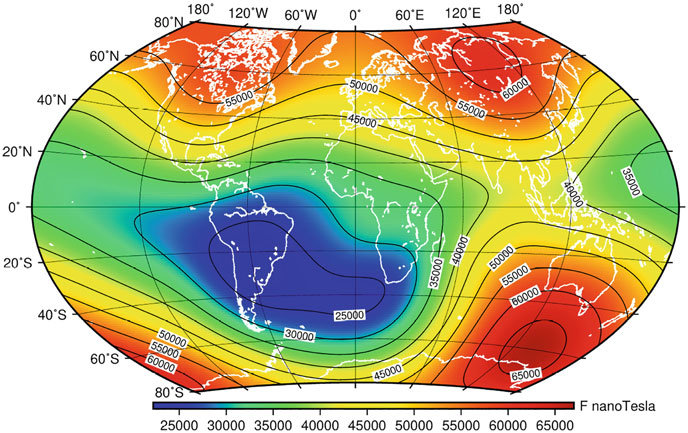
\includegraphics[width = 10cm]{Figures/IGRF-13th.png}
	\caption{The magnitude of geomagnetic field according to the 13th generation of the IGRF model~\cite{koskinen2022radiation}.}
	\label{fig:IGRF13th}
\end{figure*}

\section{Sensor models}
The positioning of the sensors on the satellite is necessary to meet mission requirements. The exact position of the sensors also impact the modelling of the anomalies on the sensors. Therefore, each sensors position on the satellite is provided as well as the measured vector of each sensor. It is further assumed that each sensor has a zero-mean Guassian noise and consequently, the low frequency noise such as drift is negligible. The sensor measurement in the SBC frame, $\mathbf{v}_{\mathcal{B}}$,  can be calculated as
\begin{equation}
\mathbf{v}_{\mathcal{B}} = \boldsymbol{A}_{\mathcal{O}}^{\mathcal{E}} \mathbf{v}_{\mathcal{I}} + \mathbf{m}_v,
\end{equation}
where $\mathbf{m}_v$ is the measurement noise of the current sensor and $\mathbf{v}_{\mathcal{I}}$ is the reference ORC vector. The measured unit vectors of the sun as an example of the sensor measurements is shown in Figure~\ref{fig:SunSensorPlot} where the grey background sections of the graphs are the eclipse periods, while the sections with the white background is the sunlit phase of the orbit.

\begin{figure}[!htb]
	\centering
	\def\pgfwidth{7cm}
	\import{Figures/TexFigures/Predictor-None/Isolator-None/Recovery-None/EARTH_SUN-ORC-General CubeSat Model/None/}{Sun.pgf}
	
	\caption{Sun vector in SBC}
	\label{fig:SunSensorPlot}
\end{figure}

%\begin{figure}[!htb]
%	\centering
%	\def\pgfwidth{7cm}
%	\import{Figures/TexFigures/Predictor-None/Isolator-None/Recovery-None/EARTH_SUN-ORC-General CubeSat Model/None/}{Earth_large.pgf}
%	
%	\caption{Earth vector in SBC}
%	\label{fig:EarthSensorPlot}
%\end{figure}
%
%\begin{figure}[!htb]
%	\centering
%	\def\pgfwidth{7cm}
%	\import{Figures/TexFigures/Predictor-None/Isolator-None/Recovery-None/EARTH_SUN-ORC-General CubeSat Model/None/}{Magnetometer_large.pgf}
%	
%	\caption{Magnetometer in SBC}
%	\label{fig:MagnetometerPlot}
%\end{figure}

\section{Disturbance models}
\label{section: disturbance models}
During orbit a satellite is exposed to various disturbance torques. It is these torques that cause the modelled attitude to differ from the actual attitude. Therefore, these torques are modelled and are assumed to influence the attitude of the satellite continuously. Other disturbances that occur only with anomalies are discussed in Chapter~\ref{chap:Anomalies}. Some disturbances are excluded from the simulation environment and only the major sources of disturbance torques are modelled and discussed.

The first disturbance torque is that of the gyroscopic coupling which can be calculated with
\begin{equation}
\mathbf{N}_{gyro} = \boldsymbol{\dot{\omega}}_\mathcal{B}^\mathcal{I} \times (\mathbf{I}\boldsymbol{\dot{\omega}}_\mathcal{B}^\mathcal{I} + \mathbf{h}_w),
\end{equation}
where $h_w$ is the angular momentum of the reaction wheels. The other disturbance torques are discussed in more detail below.

\subsection{Gravity Gradient}
The gravity gradient is caused by both the centrifugal force on the satellite due to the orbit around the Earth as well as the gravitational force. The part of the satellite nearest to the Earth will experience the largest gravitational force and the smallest centrifugal force of the satellite. While the part of the satellite furthest from the Earth will experience the smallest gravitational force and the largest centrifugal force. According to \cite{wertz2012spacecraft} the gravity gradient disturbance torque, $\mathbf{N}_{gg}$ can be calculated as 
\begin{equation}
\boldsymbol{N}_{gg} = 3 \, \omega_o^2 (\mathbf{z}_{\mathcal{B}} \times \mathbf{Iz}_{\mathcal{B}}).
\end{equation}
The orbit nadir vector is calculated as,
\begin{equation}
\mathbf{z}_{\mathcal{B}} = \boldsymbol{A} \begin{bmatrix} 0 & 0 & 1 \end{bmatrix}^T.
\end{equation}
Due to the design of the satellite and the positions of the solar panels, the equation for $\mathbf{N}_{gg}$ can not be simplified. The gravity gradient torque is the only torque that can be accurately modelled on-board the satellite, and therefore is also included in the model update of the EKF. $\mathbf{N}_{gg}$ in SBC is shown in Figure~\ref{fig:GravityGradientTorques}.

\begin{figure}[!htb]
	\centering
	\def\pgfwidth{10cm}
	\import{Figures/TexFigures/Predictor-None/Isolator-None/Recovery-None/EARTH_SUN-ORC-General CubeSat Model/None/}{Gravity Gradient Torques.pgf}
	
	\caption{Gravity Gradient Torque in SBC}
	\label{fig:GravityGradientTorques}
\end{figure}

\subsection{Aerodynamic Disturbance}
The aerodynamic disturbance torques are cause by air density in the atmosphere creating a force on each individual segment of the satellite~\cite{Steyn2014}. This is significant due to the low Earth orbit (LEO) of the satellite, where the atmospheric density is higher. Therefore, the aerodynamic disturbance torque, $\mathbf{N}_{aero}$ is a summation of all the torques created by the air force on each segment area, $A_i$. $\mathbf{N}_{aero}$ can therefore be calculated as

\begin{equation}
\begin{aligned}
\mathbf{N}_{aero} = \sum_{i=1}^{n}\Big(& \rho \norm{\mathbf{v}_{\mathcal{B}}}^2 A_i H \{\text{cos}(\alpha_i)\} \, \text{cos}(\alpha_i) \big(\sigma_t (\mathbf{r}_{pi} \times \mathbf{\bar{v}}_{\mathcal{B}}) \\
					 & + \big[ \sigma_nS + (2 - \sigma_n - \sigma_t) \text{cos}(\alpha_i)\big] (\mathbf{r}_pi \times \mathbf{\bar{n}}_i) \big) \vphantom{\norm{\mathbf{v}_{\mathcal{B}}}^2}\Big),
\end{aligned}
\end{equation}
where $n$ is the number of segments of the satellite. The factors that influence the aerodynamic disturbance torque is the atmospheric velocity in SBC, $\mathbf{v}_{\mathcal{B}}$, the atmospheric density, $\rho$, each segment's surface area, $A_i$, and the offset vector between the segment's centre of mass (CoM) and the centre of pressure (CoP), $\mathbf{r}_p$. $H\{x\}$ is the Heaviside function which is equal to $0$ when $x$ is smaller than $0$ and otherwise equal to $1$. $\alpha_i$ is the incidence angle of $\mathbf{v}_{\mathcal{B}}$ on segment $i$, while $\sigma_t$ is the tangential accommodation coefficient and $\sigma_n$ is the normal accommodation coefficient. $S$ is the ratio of molecular exit velocity to $\mathbf{v}_{\mathcal{B}}$ and $\mathbf{\bar{n}}_i$ is the unit inward normal vector of segment $i$ \cite{JansevanVuuren2015}.

The atmospheric density is a function of the distance from the Earth surface. The density model provided by \cite{vallado2001fundamentals} is given as 
\begin{equation}
\rho = \rho_o e^{-\frac{h(t)-h_o}{H}},
\end{equation}
where $\rho_o$ is the reference density at the reference altitude, $h_o$, and $h(t)$ is the satellite's altitude as a function of time and $H$ is the scale height. According to \cite{steyn2011CubeSat} the atmospheric density is $\frac{1}{2}\rho$ during eclipse. Furthermore $\mathbf{v}_{\mathcal{B}}$ is calculated as
\begin{equation}
\begin{aligned}
\mathbf{v}_{\mathcal{B}} &= \boldsymbol{A}_{\mathcal{O}}^{\mathcal{B}} \boldsymbol{A}_{\mathcal{E}}^{\mathcal{O}} \mathbf{v}_{\mathcal{E}} \\
\text{where}  \qquad \mathbf{v}_{\mathcal{E}} &= \begin{bmatrix} 0 \\ 0 \\ \omega_E \end{bmatrix} \times \mathbf{r}_{sat} - \mathbf{v}_{sat}.
\end{aligned}
\end{equation}

$\sigma_n$ and $\sigma_t$ are both assumed to be equal to 0.8, while $S$ is $\num{0.8}$~\cite{steyn2011CubeSat}. From these equations the aerodynamic disturbance can be calculated and is shown in Figure~\ref{fig:AerodynamicTorques}.
\begin{figure}[!htb]
	\centering
	\def\pgfwidth{10cm}
	\import{Figures/TexFigures/Predictor-None/Isolator-None/Recovery-None/EARTH_SUN-ORC-General CubeSat Model/None/}{Aerodynamic Torques.pgf}
	
	\caption{Aerodynamic Torques in SBC}
	\label{fig:AerodynamicTorques}
\end{figure}

\subsection{Wheel Imbalance}
The reaction wheel imbalance is considered to be the most significant disturbance on the reaction wheel and consequently, only this disturbance torque is modelled for this simulation~\cite{bialke1998high}. Although reaction wheels are manufactured with low tolerances the reaction wheel will have a slight imbalance, since the mass of the reaction wheel will not be perfectly uniform and evenly displaced. 

The static imbalance of the reaction wheel is caused by the reaction wheel CoM offset from the rotational axis. Therefore, to model the static imbalance of the reaction wheels it is assumed that the unevenly distributed mass of the reaction wheel can be simplified to a point mass, $m$, a distance, $r$ from the rotational axis as shown in Figure~\ref{fig:StaticImbalance}. The static imbalance, $U_s$ is equal to $mr$ and this value is provided by the reaction wheel manufacturers.

\begin{figure}[!htb]
	\centering
	\def\svgwidth{10cm}
	\import{Figures/}{StaticImbalance.pdf_tex}
	\caption{Static Imbalance}
	\label{fig:StaticImbalance}
\end{figure}

To determine the resulting torque from the wheel imbalance the torque generated by each wheel is individually calculated. Consequently, for the reaction wheel in direction $\bar{x}_\mathcal{B}$, $RW_{\bar{x}_\mathcal{B}}$, the force, $F_{s\bar{x}_\mathcal{B}}$, generated by $U_s$ is dependent on the the angular rate, $\omega$, of the reaction wheel as well as the current position of $m$. Therefore, $F_{s\bar{x}_\mathcal{B}}$ can be expressed as

\begin{equation}
\mathbf{F}_{s\bar{x}_\mathcal{B}} = U_s\omega^2 \begin{bmatrix} 0 \\ \text{sin}(\omega t + \phi_s) \\ \text{cos}(\omega t + \phi_s)\end{bmatrix},
\end{equation}

where the current angle of $m$ is defined as $\omega t + \phi_s$, with $\phi_s$ as an arbitrary phase and for the sake of simplification is set to $0$. With $F_{s\bar{x}_\mathcal{B}}$ exerted on $RW_{\bar{x}_\mathcal{B}}$ known, the torque on the satellite can be calculated with the known position vector, $\mathbf{w}_{\bar{x}_\mathcal{B}}$, of $F_{s\bar{x}_\mathcal{B}}$ to the satellite CoM. Therefore, $N_{s\bar{x}_\mathcal{B}}$ can be calculated as

\begin{equation}
\mathbf{N}_{s\bar{x}_\mathcal{B}} = \mathbf{w}_{\bar{x}_\mathcal{B}} \times F_{s\bar{x}_\mathcal{B}}.
\end{equation}

This is calculated for each reaction wheel to determine the resulting static imbalance disturbance torque on the satellite. Another aspect of the reaction wheel imbalance is also modelled, namely the dynamic imbalance. The dynamic imbalance is caused by the principal inertia of the reaction wheel being misaligned with the rotational axis. This can be simplified to two equal point masses, $m$, with an axial displacement, $d$, and distance, $r$, from the rotational axis. These two masses are $\num{180}^o$ apart with respect to the rotational axis and consequently create two forces equal in magnitude and in opposite directions. The dynamic imbalance is graphically represented in Figure~\ref{fig:DynamicImbalance}.

\begin{figure}[!htb]
	\centering
	\def\svgwidth{10cm}
	\import{Figures/}{DynamicImbalance.pdf_tex}
	\caption{Dynamic Imbalance}
	\label{fig:DynamicImbalance}
\end{figure}

The dynamic wheel imbalance torque, $\mathbf{N}_{d\bar{x}_\mathcal{B}}$, for $RW_{\bar{x}_\mathcal{B}}$ can be calculated as 
\begin{equation}
\mathbf{N}_{d\bar{x}_\mathcal{B}} = U_d\omega^2 \begin{bmatrix} 0 \\ \text{sin}(\omega t + \phi_d) \\ \text{cos}(\omega t + \phi_d)\end{bmatrix}.
\end{equation}
where $U_d = mrd$ as the dynamic imbalance. Both $U_d$ and $U_s$ are provided by the manufacturer and based on the reaction wheel, RW-0.06 from Sinclair Interplanetary, $U_d = 2.08e^{-9}$ and $U_s = 2.08e^{-7}$. The net wheel imbalance torque from both the static and dynamic wheel imbalance is provided in Figure~\ref{fig:Wheel disturbance Torques}.

\begin{figure}[!htb]
	\centering
	\def\pgfwidth{10cm}
	\import{Figures/TexFigures/Predictor-None/Isolator-None/Recovery-None/EARTH_SUN-ORC-General CubeSat Model/None/}{Wheel disturbance Torques.pgf}
	
	\caption{Wheel disturbance torques in SBC}
	\label{fig:Wheel disturbance Torques}
\end{figure}

\section{Attitude Determination}
This section discusses the estimation algorithm for attitude estimation of the satellite. This is done with the EKF, which utilizes the sensor measurements as well as modelled vectors according to underlying physics to estimate the current attitude. The EKF is highly sensitive to sensor anomalies and actuator failures and this section provides the background knowledge to the fundamentals of the EKF.

\subsection{Extended Kalman Filter}
The implementation of the estimated kalman filter \emph{EKF} is for estimation of the current satellite attitude with sensor fusion of the magnetometer, star tracker, sun sensor and nadir sensor to accurately estimate the attitude and rotation rate of the satellite. The EKF will be used due to the non-linear nature of the system. The EKF consists of two fundamental parts, the model update and the measurement update. The general form for a system model can be expressed as

\begin{equation}
	\dot{x_t} = \mathbf{f}(x_t) + s_t
\end{equation}

where $\mathbf{f}(x_t)$ is a non-linear function of $x_t$. The state vector, $x$, for the full 7-state EKF consists of the quaternion vector, $q$ and the inertial-referenced angular velocity, $\boldsymbol{\omega}_{\mathcal{B}}^{\mathcal{I}}$.

\begin{equation}
	x = [q, \boldsymbol{\omega}_{\mathcal{B}}^{\mathcal{I}}]^T
\end{equation}

The estimated state vector $x$ will be denoted as $\hat{x}$ and the estimated vector before and after the measurement update will be indicated with a superscript $'-'$ and $'+'$ respectively. To calculate the model update the dynamics and kinematics of the system model is used to calculate both $\boldsymbol{\omega}_{\mathcal{B}}^{\mathcal{I}}$ and $q$. The integration method used in the simulation is the 4th order Runge-Kutta method to solve the differential equations. The integration method is shown in Algorithm~\ref{alg: Runge-Kutta} where $(\hat{\omega}_{\mathcal{B}}^{\mathcal{I}})_k^-$ is calculated for the first step of the model update.

\begin{algorithm}[!htb]
	\caption[Runge-Kutta]{Runge-Kutta 4th order Algorithm at time $k$}
	\label{alg: Runge-Kutta}
	\begin{algorithmic}[1]
		\State Satellite Body Inertia $\mathbf{J} = \begin{bmatrix}
			0.4 & 0 & 0\\
			0 & 0.45 & 0 \\
			0 & 0 & 0.3
		\end{bmatrix}$
		\State Timestep ($T_s$) $= 1s$
		\State Number of iterations ($I$) $= 10$
		\State Step size $h = \frac{T_s}{h}$
		\State Disturbance torques $N_d = N_{gg} - N_{gyro} $ % + N_{aero} + N_{rw}$
		\State Control torques $N_c = N_m - N_w$
		\State $\mathbf{N} = N_c + N_d$
		\For{\texttt{$n \in I$}}
		\State \texttt{$k_1 = h(\mathbf{J^{-1}}\mathbf{N})$}
		\State \texttt{$k_2 = h(\mathbf{J^{-1}}\mathbf{N} + \frac{k1}{2})$}
		\State \texttt{$k_3 = h(\mathbf{J^{-1}}\mathbf{N} + \frac{k_2}{2})$}
		\State \texttt{$k_4 = h(\mathbf{J^{-1}}\mathbf{N} + k_3)$}
		\State \texttt{$\omega_{n+1}=\omega_n + \frac{k_1}{6} + \frac{k_2}{3} + \frac{k_3}{3} + \frac{k_4}{6}$}
		\EndFor
		\State $(\hat{\omega}_{\mathcal{B}}^{\mathcal{I}})_k^- = \omega_{n+1}$
		\State \textbf{return} $(\hat{\omega}_{\mathcal{B}}^{\mathcal{I}})_k^-$
	\end{algorithmic}
\end{algorithm}
where $N_{gg}$, gravity gradient disturbance torque, $N_{aero}$, aerodynamic disturbance torque, $N_{rw}$, reaction wheel disturbance torque, $N_{gyro}$, gyroscopic torque, $N_m$, magnetic control torque and $N_w$, reaction wheel control torque, are modelled according to \cite{JansevanVuuren2015}. 

%\begin{equation}
%	f(x,y) = \mathbf{J^{-1}}\big((N_m)_{k-1} - (N_w)_{k-1} - (N_{gg})_{k-1} - (N_{gyro})_{k-1} \big)
%\end{equation}
The calculation for the $\hat{q}_k^-$ is done with Eq~\ref{eq:q-propagation} \cite{JansevanVuuren2015}

\begin{equation}
	\begin{aligned}
		\hat{q}_k^- &= \left[\text{cos}(k_q)\mathbf{I}_{4x4} + \frac{1}{\lVert (\hat{\omega}_B^O)_k^- \rVert} \text{sin}(k_q) \mathbf{\Omega}_k^- \right] \hat{q}_{k-1}^+ \\ \\
		\text{where } k_q &= \frac{Ts}{2} \lVert (\hat{\omega}_B^O)_k^- \rVert \\ \\
		(\hat{\omega}_B^O)_k^- &= (\hat{\omega}_{\mathcal{B}}^{\mathcal{I}})_k^- - \hat{\boldsymbol{A}} \begin{bmatrix} 0 & -(\omega_k) & 0\end{bmatrix}^T \\
		&= \begin{bmatrix} \hat{\omega}_{ox} & \hat{\omega}_{oy}  & \hat{\omega}_{oz} \end{bmatrix}^T \\ \\
		\lVert (\hat{\omega}_B^O)_k^- \rVert &= \sqrt{\hat{\omega}_{ox}^2 + \hat{\omega}_{oy}^2 + \hat{\omega}_{oz}^2} \\ \\
		\text{and } \mathbf{\Omega}_k^- &= \begin{bmatrix} 
			0 & \hat{\omega}_{oz} & -\hat{\omega}_{oy} & \hat{\omega}_{ox} \\
			-\hat{\omega}_{oz} & 0 & \hat{\omega}_{ox} & \hat{\omega}_{oy}			\\
			\hat{\omega}_{oy} & -\hat{\omega}_{ox} & 0 & \hat{\omega}_{oz}			\\
			-\hat{\omega}_{ox} & -\hat{\omega}_{oy} & -\hat{\omega}_{oz} & 0			\\
		\end{bmatrix}
	\end{aligned}
	\label{eq:q-propagation}
\end{equation}

The estimated state vector, $\hat{x}_k^-$ can now be expressed as 

\begin{equation}
	\hat{x}_k^- = \begin{bmatrix} (\hat{\omega}_{\mathcal{B}}^{\mathcal{I}})_k^- & \hat{q}_k^-\end{bmatrix}
\end{equation}

$Q_k$ is the covariance matrix representing the discrete system noise and is assumed to be zero-mean and Guassian. $\Phi_k$ is the discrete system perturbation model. $H_k$ is the discrete measurement perturbation Jacobian Matrix. $\mathbf{R}_k$ is the measurement noise covariance matrix. The state covariance matrix $P_k$ can be propagated with Eq~\ref{eq:P_k}.

\begin{equation}
	\mathbf{P}_k^- = \Phi_k \mathbf{P}_{k-1}^+ \Phi_k ^T
	\label{eq:P_k}
\end{equation}
The $\mathbf{e}_k$ calculated with Eq~\ref{eq:errorVector}

\begin{equation}
	\mathbf{e}_k = v_{meas,k} - \hat{\boldsymbol{A}}_k^- v_{model,k}
	\label{eq:errorVector}
\end{equation}

where $v_{meas,k}$ is the measured vector in $\mathbf{\mathcal{B}}$ and $v_{model,k}$ is the modelled $\mathbf{\mathcal{O}}$ vector. The gain matrix $\mathbf{K}_k$ is used to determine the the influence of $\mathbf{e}_k$ on updated state vector, $\hat{x}_k^+$. $\mathbf{K}_k$ can be calculated as 

\begin{equation}
	\mathbf{K}_k = \mathbf{P}_k^- (\mathbf{H}_k^-)^T \left[\mathbf{H}_k^- \mathbf{P}_k^- (\mathbf{H}_k^-)^T + \mathbf{R}_k \right]^{-1}
\end{equation}
after which the updated state vector can be calculated with Eq~\ref{eq:UpdatedStateVector}
\begin{equation}
	\hat{x}_k^+ = \hat{x}_k^- + \mathbf{K}_k \mathbf{e}_k
	\label{eq:UpdatedStateVector}
\end{equation}

The state covariance matrix can then be updated as

\begin{equation}
	\mathbf{P}_k^+ = \left[\mathbf{I}_{7 \times 7} - \mathbf{K}_k \mathbf{H}_k^+ \right]\mathbf{P}_k \left[\mathbf{I}_{7 \times 7} - \mathbf{K}_k \mathbf{H}_k^+ \right] + \mathbf{K}_k \mathbf{R}_k \mathbf{K}_k^T
	\label{eq:Updated_P_k}
\end{equation}

During the measurement update of $\hat{x}_k^-$ with the error of $v_{meas,k}$ and $v_{model,k}$, the $\hat{x}_k^+$ is largely affected by anomalous behaviour in the sensor measurements. The sensitivity of the Kalman filter to this behaviour as well as related work will be discussed in section~\ref{subsection:SensitivityOfKalmanFilter}.

\begin{figure}[!htb]
	\centering
	\def\pgfwidth{10cm}
	\import{Figures/TexFigures/Predictor-None/Isolator-None/Recovery-None/EARTH_SUN-ORC-General CubeSat Model/None/}{Estimation Metric.pgf}
	
	\caption{Estimation Metric}
	\label{fig:Estimation Metric}
\end{figure}


\section{Attitude Control}
To ensure that the satellite is able to satisfy the mission requirements, control of the satellite attitude is required. Therefore, the satellite's payload must be in the direction of the Earth during eclipse and the solar panels should be pointing in the direction of the sun during the sunlit phase. For this control a quaternion feedback controller of the reaction wheels is implemented and a momentum dumping with the magnetorquers is implemented to ensure that the wheel disturbance remains within reasonable boundaries.

\subsection{Quaternion Feedback Controller}
\label{section: Quaternion Feedback Controller}
To ensure that the satellite is in the desired orientation the reaction wheels are used. To ensure stable control in all three axes \cite{wie1989quarternion} the quaternion feedback reaction wheel controller is implemented. The controller is designed from the estimated orientation and angular velocity, while ignoring disturbance torques. Eq~\ref{Eq-EulerDynamic} without the disturbance torques becomes
\begin{equation}
\mathbf{J}\dot{\boldsymbol{\omega}_{\mathcal{B}}^{\mathcal{I}}} = -\mathbf{N}_w - \mathbf{N}_{gyro}
\end{equation}
To calculate the required torque, $\mathbf{N}_{w,req}$, the definition according to \cite{steyn2008attitude} for all cases at time step, $k$, is given as
\begin{equation}
	\mathbf{N}_w(k) = K_{PI}\mathbf{Jq}_{err}(k) + K_{DI}\mathbf{I}\hat{\boldsymbol{\omega}}_B^O - \hat{\boldsymbol{\omega}}_{\mathcal{B}}^{\mathcal{I}}(k) \times [\mathbf{J}\hat{\boldsymbol{\omega}}_{\mathcal{B}}^{\mathcal{I}}(k) + \mathbf{h}_{w}(k)]
\end{equation}
where $\mathbf{h}_{w}(k)$ is the measured angular momentum of the wheels, the control gains are defined as
\begin{equation}
	\begin{aligned}
		K_{PI} &= 2 \omega_n^2\\
		K_{DI} &= 2 \zeta \omega_n \\
	\end{aligned}
	\label{eq:controlGain}
\end{equation}
the quaternion error is calculated with the quaternion difference operator, $\Theta$, as
\begin{equation}
	\begin{aligned}
		\mathbf{q}_{err}(k) &= \mathbf{q_c}(k) \Theta \hat{\mathbf{q}}(k) \\
		\begin{bmatrix} 
			q_{1e} \\
			q_{2e} \\
			q_{3e} \\
			q_{4e}
		\end{bmatrix} &= \begin{bmatrix} 
			q_{4c} & q_{3c} & -q_{4c} & -q_{4c} \\
			-q_{3c} & q_{4c} & q_{1c} & -q_{2c} \\
			q_{2c} & - q_{1c} & q_{4c} & -q_{3c} \\
			q_{1c} & q_{2c} & q_{3c} & q_{4c}
		\end{bmatrix}
		\begin{bmatrix} 
			\hat{q}_1 \\
			\hat{q}_2 \\
			\hat{q}_3 \\
			\hat{q}_4
		\end{bmatrix}
	\end{aligned}
	\label{eq:quaternionError}
\end{equation}
where $\hat{\mathbf{q}}$ is the current estimated quaternion and $q_{c}$ is the command quaternion which is $\begin{Bmatrix}
	0 & 0 & 0& 1
\end{Bmatrix}^T$ during eclipse and during the sun following phase, the attitude command according to \cite{chen2000ground} can be calculated as 
\begin{equation}
	\mathbf{q}_c = \begin{bmatrix}
		\mathbf{u}_c \text{sin}(\frac{\delta}{2}) \\
		\text{cos}(\frac{\delta}{2})
	\end{bmatrix},
\end{equation}
where 
\begin{equation}
	\mathbf{u}_c = \frac{\mathbf{u}_{sp}^{\mathcal{B}} \times \mathbf{s}_o}{\norm{\mathbf{u}_{sp}^{\mathcal{B}} \times \mathbf{s}_o}}.
\end{equation}
$\mathbf{s}_o$ is the measured unit sun vector in ORC, and the main solar panel's position is denoted as a unit vector, $\mathbf{u}_{sp}^{\mathcal{B}}$. The angle between $\mathbf{u}_{sp}^{\mathcal{B}}$ and $\mathbf{s}_o$, $\delta$, can be calculated with the vector dot-product. This can then be used as the reference for the control. The reference $\boldsymbol{\omega}_{\mathcal{B}}^{\mathcal{I}}$ is always $[0, 0, 0]$. 

\begin{figure}[!htb]
	\centering
	\def\pgfwidth{10cm}
	\import{Figures/TexFigures/Predictor-None/Isolator-None/Recovery-None/EARTH_SUN-ORC-General CubeSat Model/None/}{Pointing Metric.pgf}
	
	\caption{Pointing Metric}
	\label{fig:Pointing Metric}
\end{figure}

\subsection{Momentum Dumping}
Momentum dumping is crucial to ensure that the wheel disturbance does not cause the system to become unstable. Momentum dumping is implemented during eclipse after the satellite is in a stable nadir-pointing attitude. The momentum dumping is implemented with magnetic torquers based on a Cross-Product controller. 

The magnetic dipole moment $\mathbf{M}$ is calculated as 
\begin{equation}
\mathbf{M} = \frac{\mathbf{e} \times \mathbf{B}}{\norm{\mathbf{B}_b}^2}
\end{equation}
where $\mathbf{B}_b$ is the geomagnetic field and the error vector, $\mathbf{e}$ can be calculated as
\begin{equation}
\mathbf{e} = -K_w(\mathbf{h_w} - \mathbf{h_w,ref})
\end{equation}
where $K_w$ is a positive gain. This momentum dumping is implemented $200s$ after sun-following phase is implemented, to ensure stable control and reduce the momentum in the reaction wheels. The magnetorquers torques are shown in Figure~\ref{fig:Magnetic Control Torques} and it is evident that when the satellite control changes from eclipse to sunlit and from sunlit to eclipse the magnetorquers torques increase to compensate for the increase in reaction wheel torques and to minimise the dynamic reaction wheel disturbance.

\begin{figure}[!htb]
	\centering
	\def\pgfwidth{10cm}
	\import{Figures/TexFigures/Predictor-None/Isolator-None/Recovery-None/EARTH_SUN-ORC-General CubeSat Model/None/}{Magnetic Control Torques.pgf}
	
	\caption{Magnetic Control Torques}
	\label{fig:Magnetic Control Torques}
\end{figure}


%\section{Constellations}
%Explain the design of the satellite constellations and the algorithms to run communicate between satellites.
%
%\begin{algorithm}
%	
%	\SetKwInOut{Input}{Input}
%	\SetKwInOut{Output}{Output}
%	
%	\SetKwData{Left}{left}
%	\SetKwData{This}{this}
%	\SetKwData{Up}{up}
%	\SetKwFunction{Union}{Union}
%	\SetKwFunction{FindCompress}{FindCompress}
%	
%	\Indm
%	\Input{Description of the input to the algorithm.}
%	\Output{Description of the output from the algorithm.}
%	\Indp
%	
%	\BlankLine
%	
%	\emph{Initialize hyperparameters}\;
%	Get initial data from satellite\\
%	Update positions of each satellite\\
%	\For{$i\leftarrow 1$ \KwTo $N$}{
%		Determine $k$-nearest satellites to $satellite_i$ from the positions\\
%		Select data from nearest satellites\\
%		Send nearest satellites predictions and data to $satellite_i$\\
%		Retrieve data from $satellite_i$ and fault predictions of $k$-nearest satellites\\
%	}
%	Update position of $satellite_i$\\
%	Update data of $satellite_i$
%	
%	\caption[Do not end short caption with full-stop]{Algorithm example}
%	\label{alg}
%	
%\end{algorithm}


%\section{Typical Faults}
%For the simulation of the satellite and the induced faults to train and test various anomaly detection methodologies a database of typical faults is required. \cite{tafazoli2009study} made a study of the percentage of failure per subsystem. 
%
%\subsection{Probability of Fault Occurence}
%The occurrence of a fault depends on the reliability of that equipment. \cite{Guo2014} studied the reliability of small satellites and calculated the parameters for the Weibull distribution based on real data. To model the probability of a fault to occur the probability density function is used \cite{Jones2017}.
%
%This probability however is small and for the training of the system the data is too sparse for the computational abilities of any regular PC. Thus the probability of a failure during training is fixed to $1/1000000$ to produce the data required for the anomaly detection with a million test samples.
%
%\subsection{Set of faults}
%A set of typical faults for the ADCS is shown in Table~\ref{ADCS fault table}. 
%
%\newpage
%\begin{sidewaystable}[]
%	\label{ADCS fault table}
%	\begin{tabular}{|l|c|l|l|l|l|}
%		\hline
%		\multicolumn{6}{|c|}{\textbf{Internal Faults}} \\ \hline
%		\textbf{Fault classes} &
%		\multicolumn{1}{l|}{\textbf{\begin{tabular}[c]{@{}l@{}}Failure rate \\ per hour\end{tabular}}} &
%		\textbf{Fault causes} &
%		\textbf{References} &
%		\textbf{Possible effect} &
%		\textbf{Possible permutations} \\ \hline
%		\multirow{4}{*}{Reaction wheels} &
%		\multicolumn{1}{l|}{\multirow{4}{*}{2.5E-7 \cite{Spilhaus1987}}} &
%		\begin{tabular}[c]{@{}l@{}}Reaction wheel electronics \\ fail\end{tabular} &
%		\cite{allen2012satellite} \cite{Jacklin2019} &
%		\begin{tabular}[c]{@{}l@{}}Does not respond \\ to control inputs\end{tabular} &
%		\begin{tabular}[c]{@{}l@{}}Momentum remains the same \\ or decreases slightly due to \\ friction\end{tabular} \\ \cline{3-6} 
%		&
%		\multicolumn{1}{l|}{} &
%		Overheated reaction wheel &
%		\cite{Wintoft} &
%		Decrease in speed &
%		1\% of initial speed per second \\ \cline{3-6} 
%		&
%		\multicolumn{1}{l|}{} &
%		\begin{tabular}[c]{@{}l@{}}Catastrophic failure (cause \\ unknown)\end{tabular} &
%		\cite{Choi2011} &
%		Stops rotating &
%		0 \\ \cline{3-6} 
%		&
%		\multicolumn{1}{l|}{} &
%		\begin{tabular}[c]{@{}l@{}}Increase in rotation speed \\ (Unknown cause)\end{tabular} &
%		\begin{tabular}[c]{@{}l@{}}Gerhard Janse \\ van Vuuren\end{tabular} &
%		\begin{tabular}[c]{@{}l@{}}Wheel speed \\ increases\end{tabular} &
%		\begin{tabular}[c]{@{}l@{}}Between 90-100\% of maximum \\ wheel speed\end{tabular} \\ \hline
%		Magnetorquers &
%		\multicolumn{1}{l|}{ADCS fault table8.15E-9 \cite{Spilhaus1987}} &
%		Polarities are inverted &
%		\cite{Crowell2011} &
%		Incorrect rotation &
%		\\ \hline
%		\multirow{2}{*}{Magnetometers} &
%		\multicolumn{1}{l|}{\multirow{2}{*}{8.15E-9 \cite{Spilhaus1987}}} &
%		Unknown &
%		\begin{tabular}[c]{@{}l@{}}Gerhard Janse \\ van Vuuren\end{tabular} &
%		Stops reacting &
%		\begin{tabular}[c]{@{}l@{}}Provides no feedback or the \\ output remains constant\end{tabular} \\ \cline{3-6} 
%		&
%		\multicolumn{1}{l|}{} &
%		\begin{tabular}[c]{@{}l@{}}Magnetometers and magne-\\ torquers interfered with \\ each other\end{tabular} &
%		\cite{Jacklin2019} &
%		\begin{tabular}[c]{@{}l@{}}Noise on magneto-\\ meters and noise \\ on control of mag-\\ netorquers\end{tabular} &
%		\begin{tabular}[c]{@{}l@{}}Between x3 and x5 times the \\ normal noise magnitude \\ Guassian distribution\end{tabular} \\ \hline
%		Earth Sensor &
%		- &
%		Unknown &
%		\cite{Robertson2019} &
%		\begin{tabular}[c]{@{}l@{}}Noisy Earth Sensor \\ effected pointing \\ accuracy\end{tabular} &
%		\begin{tabular}[c]{@{}l@{}}Between x5 and x10 times the \\ normal sensor noise based on \\ Guassian distribution\end{tabular} \\ \hline
%		\multirow{2}{*}{Sun sensor} &
%		\multirow{2}{*}{-} &
%		\begin{tabular}[c]{@{}l@{}}Cross-wired during instal-\\ lation\end{tabular} &
%		\cite{Crowell2011} &
%		\begin{tabular}[c]{@{}l@{}}Erroneous \\ measurements\end{tabular} &
%		Uniform random values \\ \cline{3-6} 
%		&
%		&
%		Unknown &
%		\cite{Jacklin2019} &
%		Sun sensor fails &
%		output is 0 \\ \hline
%		Star tracker &
%		- &
%		\begin{tabular}[c]{@{}l@{}}Shutter on star tracker is \\ closed\end{tabular} &
%		\cite{Crowell2011} &
%		Star tracker fails &
%		output is 0 \\ \hline
%		Overall control &
%		- &
%		\begin{tabular}[c]{@{}l@{}}Incorrect control law or \\ variation \\ thereof\end{tabular} &
%		\begin{tabular}[c]{@{}l@{}}Gerhard Janse \\ van Vuuren\end{tabular} &
%		\begin{tabular}[c]{@{}l@{}}Angular velocity \\ suddenly increases \\ or decreases or \\ oscillation results\end{tabular} &
%		\begin{tabular}[c]{@{}l@{}}Increase to 75 - 100\% \\ Decrease to 0 - 25\%\\ Oscillates\end{tabular} \\ \hline
%		\multirow{3}{*}{\begin{tabular}[c]{@{}l@{}}Common data \\ transmission errors\end{tabular}} &
%		\multirow{3}{*}{-} &
%		Sign flip &
%		\cite{Crowell2011} &
%		Processor-based &
%		\begin{tabular}[c]{@{}l@{}}Processor outputs and/or \\ inputs experience a sign flip\end{tabular} \\ \cline{3-6} 
%		&
%		&
%		Bit flip &
%		N/A &
%		&
%		\begin{tabular}[c]{@{}l@{}}Processor outputs and/or \\ inputs experience a bit flip flip\end{tabular} \\ \cline{3-6} 
%		&
%		&
%		Insertion of zeros &
%		\cite{Jacklin2019} &
%		&
%		\begin{tabular}[c]{@{}l@{}}Processor outputs and/or inputs \\ experience an insertion of a zero\end{tabular} \\ \hline
%		\begin{tabular}[c]{@{}l@{}}Possible sensors \\ errors\end{tabular} &
%		- &
%		Unknown &
%		N/A &
%		High sensor noise &
%		\begin{tabular}[c]{@{}l@{}}Between x5 and x10 times the \\ normal sensor noise based on \\ Guassian distribution\end{tabular} \\ \hline
%	\end{tabular}
%\end{sidewaystable}
%
%\newpage